\noindent \texttt{V: 04-11-2022 11:33:00}

\section*{Experimento: - LEI DE OHM}
\section*{Teoria}

A aplicação de uma diferença de potencial elétrico V em um fio faz aparecer, nele, uma \textbf{corrente elétrica $I$}. A \textbf{resistência elétrica $R$} entre dois pontos quaisquer de um condutor é definida pela equação
\begin{equation}
    R = \frac{V}{I}
    \label{eq:R}
\end{equation}

\noindent A resistência $R$ é uma característica do fio como um todo, ou seja, depende do comprimento, da espessura e do material de que ele é feito. Por outro lado, a grandeza \textbf{resistividade ($\rho$)} é uma propriedade {\color{red}específica dos materiais} e depende de características microscópicas intrínsecas. Ou seja, pode-se lidar com fios de diferentes tamanhos e espessuras de um mesmo metal, cada um deles apresentando um valor diferente de resistência, porém, com a mesma resistividade. Essa grandeza informa como é a resposta microscópica do meio, ou seja, qual é a \textbf{densidade de corrente $J$} quando o meio é sujeito a um \textbf{campo elétrico $E$}. Matematicamente, tem-se esta relação microscópica:
\begin{equation}
    \rho = \frac{E}{J}
    \label{eq:rho}
\end{equation}

\noindent Como, no Sistema Internacional de Unidades (SI) as unidades de $E$ são $[V/m]$ (Volt/metro) e de $J$ são $[A/m^{2}]$ (Ampère/metro quadrado), $\rho$ é dado em $[\Omega.m]$ (ohm x metro).
No caso de um fio uniforme de comprimento $l$ e seção reta de área $A$, tem-se
\begin{equation}
    E = \frac{V}{l} \;\;\; \text{e} \;\;\; J = \frac{I}{A}
    \label{eq:EeJ}
\end{equation}

\noindent 
Combinando-se as equações \ref{eq:R}, \ref{eq:rho} e \ref{eq:EeJ}, chega-se a uma relação entre a resistência e a resistividade de um fio uniforme, dada por 
\begin{equation}
    R = \rho \frac{l}{A}
\end{equation}


\noindent Medindo-se a resistência de um fio uniforme e homogêneo em função de seu comprimento, pode-se determinar a resistividade do material de que ele é feito. Para isso, basta conhecer a área da seção reta do fio.


\section*{Prática}
	\section{Objetivos}
	
	Verificar experimentalmente a dependência da resistência em função dos seguinte parâmetros: A relação entre a voltagem aplicada  e acorrente; O Tipo de material, comprimento do fio, espessura do fio. 
	\section{Material utilizado}
	
	\begin{itemize}
		\item[a)] Fonte de Tensão e Corrente Contínua (CC);
		\item[b)] Uma Tábua didática Azheb - Lei de Ohm;
		\item[c)] Um multímetro;
		\item[d)] Dois fios ou cabos condutores;
		\item[e)] Um papel milimetrado;
		\item[f)] Uma régua ou trena ou paquímetro ou micrômetro.
		
	\end{itemize}

	\section{Procedimento experimental}
	
	\subsection{A - Relação entre a voltagem e a intensidade da corrente elétrica de um resistor}

\begin{enumerate}	
\item Monte o circuito de acordo com a figura \ref{fig:circuito-r-cc};

\begin{figure}[H]
\centering
    \begin{circuitikz}[american voltages]
    \draw %é (x1,y1) to [battery1, v=$V$] (x2,y2) uma matriz com origem no canto inferior esquerdo
      (0,0) to [battery1, v=$V$] (4,0)
      (0,2) to [ammeter, i=$I$] (4,2)
      (4,0) --  (4,2) 
      (0,0) to [R, color=red, R=$R$] (0,2)
      (-2,0) to [voltmeter, color=blue] (-2,2)
      (-2,0) --  (0,0)
      (-2,2) --  (0,2);  
    \end{circuitikz}
	\caption{Circuito CC Resistivo Básico. \textit{Fonte: Autor}.}
	\label{fig:circuito-r-cc}
\end{figure}

\item Ajuste o multímetro para atuar como amperímetro na escala para 10 A;

\item Monte o circuito, conforme o esquema da figura \ref{fig:circuito-r-cc}, com um fio de 1 m do painel, a fonte e o amperímetro (em série);  

\item Use os controles da fonte e varie a tensão entre $1\,V$ e $5\,V$, meça os valores de corrente e complete a Tabela \ref{tab:v-x-i}. {\color{red} \textsc{FAÇA AS MEDIDAS RAPIDAMENTE, PARA NÃO DANIFICAR A FONTE}};
\item Com os dados da Tabela, faça o gráfico $I \times V$. 

\item Analise o gráfico para determinar o tipo de função;

\item Qual a relação entre as grandezas envolvidas? 

\item Determine o valor médio de $V/I$;

\item Compare o erro entre o valor médio experimental calculado e o valor medido com o multímetro? 

\item Que significado físico tem $V/I$ ?

\end{enumerate}


	
	%Tabela 1
		\begin{table}[H]
			\centering
		\begin{tabular}{*{3}{|c}|}
			\hline 
			Tensão da fonte [$V$] & Corrente medida [$A$] & Cálculo $V/I \; [V/A]$\\ 
			\hline 
			1,0 & & \\ 
			\hline 
			2,0 & & \\ 
			\hline 
			3,0 & & \\ 
			\hline
			4,0 & & \\ 
			\hline 
			5,0 & & \\ 
                \hline  \hline 
			\multicolumn{2}{|r|}{\textbf{Media:}} & \\ 
				\hline 		
		\end{tabular}
			\caption{\label{tab:v-x-i} Razão entre Voltagem e Corrente em condutor.}
		\end{table}
	
	
	\subsection{B - Dependência de R em relação ao comprimento do fio}
    
    \begin{enumerate}	
	\item Monte o circuito de acordo com a figura \ref{fig:circuito-r2-cc};

\begin{figure}[H]
	\centering
    \begin{circuitikz}[american voltages]
    \draw
      (0,0) to [battery2, v=$V$] (4,0)
      (0,2) to [ohmmeter] (4,2)
      (4,0) --  (4,2) 
      (0,0) to [vR, color=red, vR=$R$] (0,2);
    \end{circuitikz}
	\caption{Circuito CC Resistivo Variável Básico. \textit{Fonte: Autor}.}
	\label{fig:circuito-r2-cc}
\end{figure}
	

    \item Ajuste o multímetro para atuar como ohmímetro;
    \item Para \textbf{um} fio do painel, conecte o multímetro e meça as diferentes resistências para diferentes comprimentos;  
    \item Anote os valores na Tabela \ref{tab:RxL};
    \item Com os dados da Tabela \ref{tab:RxL}, faça o gráfico $R \times L$;  
    \item Analise o gráfico para determinar o tipo de função;
    \item Qual a relação entre as grandezas envolvidas?
    \end{enumerate}
 
%Tabela 2
		\begin{table}[H]
			\centering
		\begin{tabu}{| X[c] | X[c] | X[c] | X[c] |}
			\hline 
			Condutor resistivo utilizado (material) e diâmetro $\oslash$(mm) &  Comprimento do fio $(m)$ & Resistência ôhmica medida  $(\Omega)$ & Quociente  $(R.A/L)$ \\ %cabeçalho
			\hline 
			Ni-Cr $\oslash \;0,36$& 0,20 &  &    \\ 
			\hline 
			Ni-Cr $\oslash \;0,36$ & 0,40 &  &    \\ 
			\hline 
			Ni-Cr $\oslash \;0,36$ & 0,60 &  &    \\ 
			\hline 
			Ni-Cr $\oslash \;0,36$ & 0,80 &  &    \\ 
			\hline 
			Ni-Cr $\oslash \;0,36$ & 1,00 &  &    \\ 
			\hline \hline 
			\multicolumn{3}{|r| }{\textbf{Média:}} & \\
			\hline 
		\end{tabu} 
			\caption{Variação da resistência em função do comprimento de um condutor $R/L$.}
			\label{tab:RxL}
		\end{table} 
  
\subsection{D - Dependência de R em relação à área da seção reta do condutor  }

\begin{enumerate}
    \item Complete a Tabela \ref{tab:RxA} abaixo para fios \textbf{com $L=1\,m$} e com diferentes materiais e áreas de seção transversal.
    \item Com os dados da Tabela \ref{tab:RxA}, faça o gráfico R x A.
    \item Analise o gráfico para determinar o tipo de função.
    \item Qual a relação entre as grandezas envolvidas?
\end{enumerate}
        
        %Tabela 3
		\begin{table}[H]
			\centering
		\begin{tabu}{| X[c] | X[c] | X[c] | X[c] |}
			\hline 
			Condutor (material) e diâmetro $\oslash \;$(m) &  Área da seção transversal $(m^{2})$ & Resistência ôhmica medida  $(\Omega)$ & Produto calculado (RxA)  \\ %cabeçalho
			\hline 
			 Ni-Cr $\oslash \;3,6 \times 10^{-4}$&  &  &    \\ 
			\hline 
			 Ni-Cr $\oslash \;5,1 \times 10^{-4}$&  &  &    \\ 
			\hline 
			 Ni-Cr $\oslash \;7,2 \times 10^{-4}$&  &  &    \\ 
			\hline
			 Fe $\oslash \;5,1 \times 10^{-4}$&  &  &    \\ 
			\hline 
		\end{tabu} 
			\caption{Variação da resistência em função do diâmetro de um condutor $R \times A$.}
			\label{tab:RxA}
		\end{table} 

    \subsection{C - Resistividade}

\begin{enumerate}
    \item Complete a Tabela \ref{tab:resistividade} abaixo para fios de mesmo material (Ni-Cr) com diferentes áreas de seção transversal (\textbf{copie da Tabela \ref{tab:RxA}});
    \item Calcule a média e compare com os valores da literatura.
\end{enumerate}    
    
    		%Tabela 4
		\begin{table}[H]
			\centering
		\begin{tabular}{|c|c|c|l|}
			\hline 
			Diâmetro $\oslash \; (m)$ & Área $[m^2]$ &  Resistência $(\Omega)$ & Resistividade $(\rho)\,[\Omega .m]$ \\ 
			\hline 
			Ni-Cr $3,6 \times 10^{-4}$ &  &  & \\ 
			\hline 
			Ni-Cr $5,1 \times 10^{-4}$ &  &  & \\ 
			\hline 
			Ni-Cr $7,2 \times 10^{-4}$ &  &  & \\ 
			\hline \hline 
			\multicolumn{3}{|r| }{\textbf{Média:}} & \\
			\hline 
		\end{tabular}
			\caption{Coeficiente de resistividade para o Nicromo (Ni-Cr)}
			\label{tab:resistividade}
		\end{table} 
		




\section{Relatório ou Exercícios}

\begin{itemize}
\item Construa o relatório apresentando os itens obrigatórios. 

\item Comente as prováveis fontes de erro. 

\item Responda as questões formuladas. 

\item Apresente os dados organizados em Tabelas. 

\item Apresente a análise dos dados e gráficos. 

\item Apresente os resultados solicitados no sistema internacional de unidades com todos os cálculos efetuados.  
	
\end{itemize}

\noindent
{\color{red} \rule{\linewidth}{0.5mm} }
\textbf{Dica:}

\noindent \texttt{ O que se espera? Algo do tipo...}


\begin{figure}[H]
	\centering
	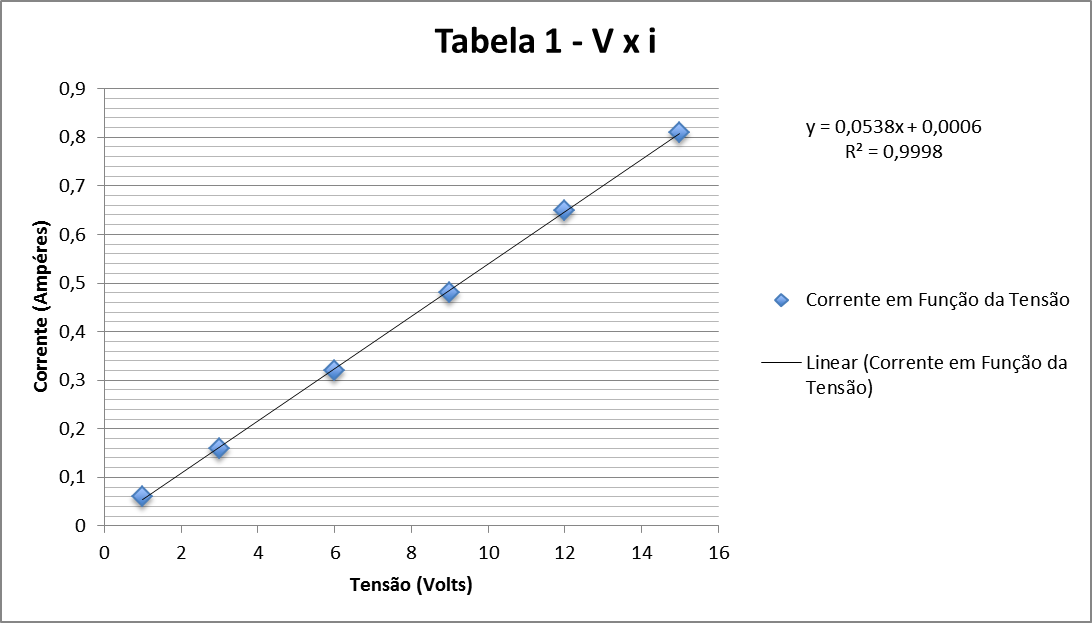
\includegraphics[scale=.4]{img/lei-de-ohm.jpg}
	\caption{$I \times V$. Fonte: Web.}
	\label{fig:imagem1}
\end{figure}

\noindent Coeficientes de Resistividade:

\noindent $\rho_{Ni-Cr} = 10,0 \times 10^{-7}\;\Omega.m$

\noindent $\rho_{Fe} = 10,0 \times 10^{-8}\;\Omega.m$






